\author{Andrei Tkachuk}

\section{Условные экстремумы ФНП}

\begin{Example}
    Найти экстремум для функции $u = x^2 + y^2$, ограниченной поверхностью $S: x + y = 1$\\
    \begin{figure}[h!]
        \noindent\centering{
            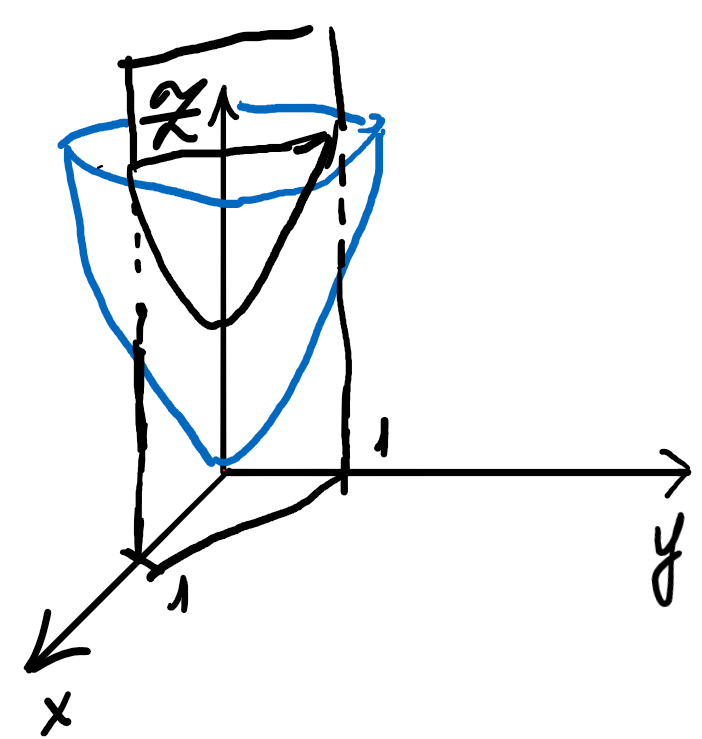
\includegraphics[width=35mm]{1_3_1.png}
            \caption{}
        }
    \end{figure}

    Решение
    \begin{align*}
        &y = 1 - x \; \Rightarrow \; u = x^2 + 1 + x^2 - 2x\\
        &u'_x = 4x - 2 = 0 &u''_x = 4 > 0\\
        &\begin{cases} 
                x = \frac{1}{2}\\
                y = \frac{1}{2}
        \end{cases} & \text{точек нет}
    \end{align*}
    Таким образом $M_0(\frac{1}{2}, \frac{1}{2})$ --- экстремум (строгий минимум)
\end{Example}
    В следующем примере предыдущий алгоритм не работает.
\begin{Example}
    Найти экстремум для функции $u = x$, ограниченной поверхностью $S: x^2 + y^2 = 1$\\
    \begin{figure}[h!]
    \noindent\centering{
        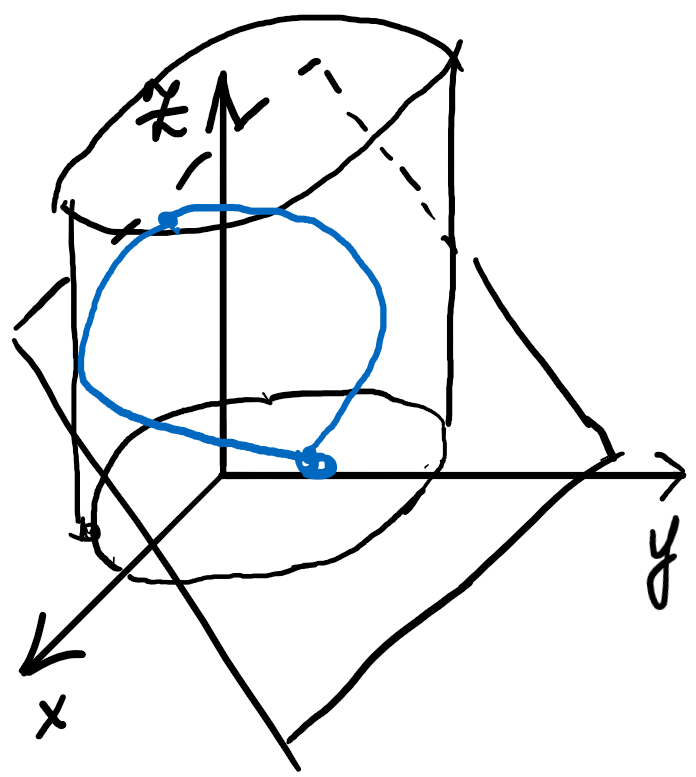
\includegraphics[width=35mm]{1_3_2.png}
        \caption{}
    }
    \end{figure}

    Если взять частную производную по $x$, то получим ($u'_x \neq 0$) что экстремум отсутствует, но по построению видно, что их два. Ошибка в том, что от "элипса" мы перешли к "отрезку" путём взятия производной.\\
    
    Чтобы избавиться от этого параметризируем $x$ и $y$ следующим образом
    \[
        \begin{cases}
        x = cos(t)\\
        y = sin(t) 
        \end{cases}
        t \in \bb{R}, \, t \in [0;\; 2\pi]
    \] 
    Тогда получим
    \begin{align*}
        &u = cos(t)\\
        &u'_t = -sin(t)\\
        &t_{min} = 0, \; t_{max} = \pi \text{, видно по построению}\\ 
        &u''_t = -cos(t)
    \end{align*}
    
\end{Example}
Таким образом, ключевым моментом является сохранение гладкости функции при взятии производных (т.е. если )

\begin{Note}[Условие связи. Условное]
    Условие свизи это функция(и) $\varphi_n(M)$, которая(ые) применяется(ются) к фукции $f(M)$, чтобы наложить ограничения (условия) на неё.
\end{Note}

\begin{Def}[Условный экстремум]
    Пусть $u = f(M) = f(x_1, \dots, x_n)$ определена в некоторой окрестности $U(M_0), \, M(x^0_1, \dots, x^0_n)$ и выполнено условие связи $S : \varphi_1(M) = 0, \dots, \varphi_k(M) = 0, \, M_0 \in S$. Тогда
        \begin{enumerate}
            \item $M_0$ --- точка локального условного минимума функции $f(M)$ при условии $M \in S \Leftrightarrow \exists \delta > 0 \; \forall M \in U_\delta(M_0) \cap S \; f(M) \geqslant f(M_0)$
            
            \item $M_0$ --- точка локального условного максимума функции $f(M)$ при условии $M \in S \Leftrightarrow \exists \delta > 0 \; \forall M \in U_\delta(M_0) \cap S \; f(M) \leqslant f(M_0)$
                        
            \item $M_0$ --- точка условного экстремума функции $f(M) \Leftrightarrow M_0$ точка условного минимума или условного максимума 
        \end{enumerate}
    Анлогичны будут рассуждения для строгого условного экстремума (помним, что он рассматривается в проколотой окрестности).
\end{Def}

\textcolor{cyan}{Повторимся, что условный экстремум отличается от обычного тем, что поиск ограничен $S$}

\begin{Def}[Формула Лагранжа задачи на усл. экстремум]
    Пусть $f(M), \varphi_1(M), \dots, \varphi_k(M)$ --- функции $n$ переменных $x_1, \dots, x_n$, определенных в $U(M_0)$. Тогда функция $L(M_i, \lambda) = f(M) + \lambda_1 \varphi_1(M) + \dots + \lambda_k \varphi_k(M)$ называется функцией Лагранжа задачи на условный экстремум функции $f(M)$ при условии $M \in S : \varphi_1 = \dots = \varphi_k = 0$
\end{Def}
\textcolor{cyan}{Формула Лагранжа позволяет связать функцию и дополнительное условие воедино, что очень удобно}

\begin{Th}[Необходимый признак условного экстремума]
    Пусть 
    \[
        f(M), \varphi_1(M), \dots, \varphi_k(M) \in C^{-1}(U(M_0))
    \] 
    и $M_0$ --- внутренняя точка гладкой части поверхности $S$ 
    \[
    S: \varphi_1(M) = 0, \dots, \varphi_k(M) = 0, \, M_0 \in S
    \]
    Обозначим через 
    \[
        L(M, \lambda) = f(M) + \lambda_1\varphi_1(M) + \dots + \lambda_k\varphi_k(M)
    \]
    функцию Лагранжа задачи на условный экстремум функции $f(M)$, где $M \in S$. Тогда, если точка $M_0$ --- условный экстремум функции $f(M)$, то существует $\lambda_0(\lambda^0_1, \dots, \lambda^0_k)$, для которой
    \[
        dL(M_0, \lambda_0) = 0, \text{ где }  M_0(x^0_1, \dots, x^0_n), \; \lambda_0(\lambda^0_1, \dots, \lambda^0_k)
    \]
\end{Th}
\begin{Proof}
    Рассмотрим следующий случай: $n = 2, \, k = 1$ (размерность пространства и количество функций задающих поверхность), то есть $u = f(x, y), \; (x, y) \in U(M_0), \; M_0(x_0, y_0), \; M_0$ --- точка условного экстремума $S : \varphi(x, y) = 0$\\
    \begin{figure}[h!]
        \noindent\centering{
            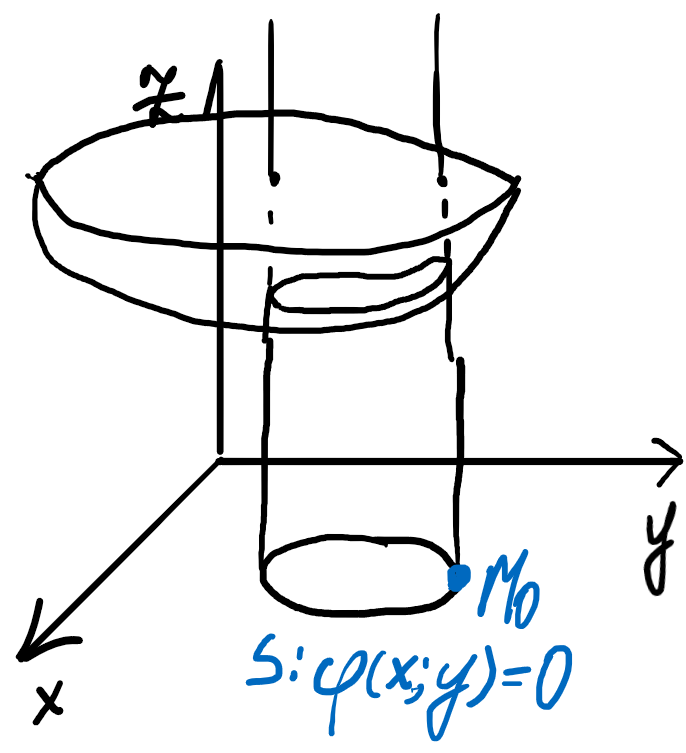
\includegraphics[width=35mm]{1_3_3.png}
            \caption{}
        }
    \end{figure}\\
    Так как $\varphi(x, y)$ --- гладкая функция, то мы можем её параметризировать
    \[
        S \begin{cases} 
            x = x(t)\\
            y = y(t)
          \end{cases}, \; t \in U(t_0)
    \]
    При этом: $M_0(x(t_0), y(t_0)), \; x(t), \, y(t) \in C'(U(t_0))$.\\
    Из этого следует, что
    \[
        \forall t \in U(t_0) \Rightarrow \varphi(x(t), y(t)) = 0
    \]
    При этом $(x'(t_0), y'(t_0)) \neq (0, 0)$, то есть параметриация "хорошая" (Важность факта можно понять из примера 2).\\
    Таким образом задача на условный экстремум переходит в задачу на обычный экстремум функции $u = f(x(t), y(t))$\\
    \textcolor{red}{Почему мы можем устроить такой переход??? Т.е. до этого у нас была $\varphi(x, y)$ и её мы параметризировали. Или мы просто сказали, что x и y можно выразить через параметр (скорее всего да, но это странный довод)?}\\
    По формуле частной производной
    \[
        u'(t) = f'_xx'_t+f'_yy'_t
    \]
    Так как $M_0$ - условный экстремум (по усл.), то $t_0$ - экстремум $u(t) \Rightarrow u'_t(t_0) = 0$.
    
    \begin{align*}
        \begin{cases}
            f'_xx'_t+f'_yy'_t = 0\\
            \varphi'_xx'_t+\varphi'_yy'_t = 0 \textcolor{red}{\text{ откуда?}}
        \end{cases}
        \begin{pmatrix}
            f'_x & f'_y\\
            \varphi'_x & \varphi'_y
        \end{pmatrix}
          = \textcolor{red}{0} \Rightarrow \frac{f'_x(M_0)}{\varphi'_x(M_0)} = \frac{f'_y(M_0)}{\varphi'_y(M_0)} = -\lambda_0\\
          \textcolor{red}{\text{Почему определитель матрицы равен нулю?}}\\
        \text{Примечание. Если знаменатель равен нулю, то и числитель будет ему равен}
    \end{align*}
    Таким образом из отношения можно получить следующию систему
    \[
        \begin{cases}
            f'_x(M_0) + \lambda_0\varphi'_x(M_0) = 0\\
            f'_y(M_0) + \lambda_0\varphi'_y(M_0) = 0\\
            \varphi(M_0) = 0 \textcolor{red}{\text{ тут не упущена производная?}}
        \end{cases}
    \]
    Которая на самом деле ни что иное как
    \[
        \begin{cases}
            L'_x(M_0, \lambda_0) = 0\\
            L'_y(M_0, \lambda_0) = 0\\
            L_\lambda(M_0) = 0 \textcolor{red}{\text{ тут не упущена производная? Как определена эта функция?}}
        \end{cases}
    \]
    Если мы сложим все три равенства то получим производную функции Лагранжа, которая равна нулю
    \[
        dL(M_0, \lambda_0) = 0
    \]
\end{Proof}

\begin{Th}[Необходимый признак усл. экстремума в общем случае]
    Пусть 
    \begin{gather*}
        \exists M(x_1, \dots, x_n), \, \exists M_0(x^0_1, \dots, x^0_n)\\
        f(M), \varphi_1(M), \dots, \varphi_k(M) \in C^2(U(M_0))\\
        L(M, \lambda) = f(M) + \lambda_1\varphi_1(M) + \dots + \lambda_k\varphi_k(M) 
    \end{gather*}
    и $\exists \lambda_0(\lambda^0_1, \dots, \lambda^0_k)$ для которой 
    \[
        dL(M_0, \lambda_0) = 0
    \]
    \textcolor{red}{Дописать!!! Тут упущенны странные вещи с матрицами}\\
    Тогда
    \begin{enumerate}
        \item $q > 0 \Rightarrow M_0$ --- точка строгого условного минимума функции
        
        \item $q < 0 \Rightarrow M_0$ --- точка строгого условного максимума функции
        
        \item $q$ --- неопределённая форма $\Rightarrow$ в $M_0$ нет экстремума 
    \end{enumerate}
\end{Th}
\begin{Proof}
    Принимаем без доказательств
\end{Proof}

\begin{Note}
    Условие $q > 0$ или $q < 0$ проверяется с помощью критерия Сильвестра. Данный факт используется для доказательства теоремы. 
\end{Note}

\begin{Note}
    По аналогии со вторым параграфом. Требуются дополнительные исследования, если второй диференциал равен нулю.
\end{Note}

\begin{Example}
    Дано:
    \[
        u = x^2 + y^2 + z^2 \; S:\: x\,y + z = 2
    \]
    Решение:
    \begin{align*}
        L = x^2 + y^2 + z^2 + 2\,\lambda
    \end{align*}
    \textcolor{red}{Дописать!!!}
\end{Example}